\documentclass[conference]{IEEEtran}
\usepackage{amsmath,amssymb,graphicx,booktabs,url}
\newcommand{\BookSpeedup}{4.87}
\newcommand{\HotMedianRange}{96.1--103.9}
\newcommand{\HotPninetyRange}{140.4--164.8}
\newcommand{\ThroughputRange}{16.08--20.37}

\title{A Reproducible In-Memory Tick-to-Trade Pipeline with Queue-Aware Synthetic Strategy Evaluation}
\author{\IEEEauthorblockN{Author information pending}\IEEEauthorblockA{Research draft; affiliation and venue metadata pending}}
\begin{document}\maketitle
\begin{abstract}
We present a reproducible evaluation of a C++20 tick-to-trade engine and its synthetic queue-aware backtester. The pipeline processes encoded market data through a book, a heuristic market maker, risk checks, an order manager and a staged order-entry frame. Repeated host measurements, preserved binned latency distributions, an independent map/list order-book comparison, byte-exact replay, paired strategy ablations, latency and queue sensitivity, and disjoint training/held-out markets provide inspectable evidence. The study corrects a histogram rank error and a test harness failure. Testing is distinguished from formal verification, in-memory latency from exchange latency, and simulator PnL from empirical trading returns. The contribution is an integrated systems artifact with transparent measurement boundaries; no new optimal-control solution or real-market profitability is established.
\end{abstract}
\begin{IEEEkeywords}tick-to-trade systems, market making, reproducible benchmarking, synthetic backtesting\end{IEEEkeywords}
\section{Scope and Prior Work}
Market-making theory studies the tradeoff between spread capture and inventory risk, including the classical Avellaneda--Stoikov framework~\cite{avellaneda2008}. Exchange latency and market design influence execution incentives~\cite{budish2015}. Neither theoretical work implies that a hand-tuned imbalance signal is an HJB-optimal strategy, or that a shared-VM microbenchmark measures an exchange round trip.

We study \texttt{rxj0102/hft}, a C++20 research engine. Its own documentation carefully limits claims to synthetic and local fake-exchange experiments. The supplied manuscript overstated those results as formal proofs, real-tape adapters, physical-memory guarantees and optimized stochastic control. This revision replaces those assertions with executable evidence. The design combines familiar components; its novelty is primarily systems integration and reproducible verification, rather than a new trading theory.

\section{Implemented Pipeline}
\subsection{Memory and Event Processing}
An encoded feed packet passes through A/B arbitration, gap detection and snapshot recovery, order-book updates, a market-making decision, pre-trade risk, order management and order-entry staging. Run-to-completion execution avoids a thread handoff in this measured path. The book uses flat price levels, pooled intrusive order nodes, a bitmap and an ID lookup table. The 32-byte node size is a compile-time check; it is not a theorem that every access avoids cache splits or misses. Memory-lock success and hugepage hints are observed runtime properties, not physical-contiguity guarantees.

A compile target checks selected hot-path headers with exceptions and RTTI disabled. Allocation/page-fault checks in the benchmark and differential state tests provide empirical assurance on exercised paths. They do not prove all executions allocation-free, race-free, bounded in wall-clock time, or safe on an exchange. The benchmark excludes NIC reception, kernel networking, TLS, JSON parsing and exchange processing.

\subsection{Strategy and Synthetic Venue}
The strategy combines a spread, order-book imbalance lean and inventory skew with risk limits. Its coefficients are engineering choices. We do not derive an optimal control or claim that imbalance has predictive power outside the generator. The backtester stages orders through the production gateway and OMS and executes them in a queue-aware synthetic venue with separate market-data, ingress and egress delays.

The synthetic generator includes informed flow that imbalance reveals. Thus the no-imbalance ablation tests whether this engineered signal is used, not whether alpha exists in historical data. Marked PnL is decomposed into spread edge, inventory mark-to-market and explicit fees. Large inventory exposure can increase simulated mean PnL without improving risk-adjusted performance. There is no modeled endogenous market impact or calibrated real-venue queue model.

\section{Corrections and Verification Design}
The original histogram selected rank $\lfloor qn\rfloor$; for odd sample counts this can fall below the stated nearest-rank quantile. We use $\lceil qn\rceil$ and add regression checks. Read-only histogram export preserves bin counts and tick-to-nanosecond calibration without adding operations to timed recording. Bins have bounded relative quantization, so these are compressed distributions rather than individual event traces.

The official Python live-tool test closed stdin then called \texttt{communicate()}, which flushed the closed stream under Python 3.12 and 3.13. Clearing the closed handle fixes the harness while retaining process, EOF and signal checks. The complete local CI includes local fakes and 28 fault drills, separate from CTest's 19 suites. Existing reference-model and replay checks are differential testing, not formal verification. Mutation rates and instruction budgets in historical documentation are not reported as newly reproduced here.

\section{Prespecified Experiments}
\subsection{Host Timing and Reference Baseline}
Five sequential release-benchmark runs each generate 300,000 requests, verify byte-exact replay against the backtest session and record warm and cold-cache distributions. Hardware, compiler flags, binaries, source hashes, timer calibration, affinity and scheduling-noise observations are retained. The final timing pass runs after other task-started CPU-heavy tests finish. The host is a shared AMD EPYC 9V74 Linux VM with a four-core quota and 32 GiB memory limit, using GCC 14 and the repository release preset. CPU isolation and fixed frequency are not guaranteed. The timer overhead is subtracted as documented by the benchmark; probe effects and VM stalls remain.

An offline operation benchmark compares the flat book with the independent \texttt{std::map}/\texttt{std::list} reference already used by tests. Five seeded tapes each contain 20,000 warmup and 200,000 timed mixed operations, with a target of 5,000 resting orders. Setup and generation are untimed. Return values and periodic state digests are compared before timing, and final digests must match. Execution order alternates across seeds. This is a book-update baseline, not an alternative complete production engine or a claim against a tuned competitor.

\subsection{Ablations and Statistics}
The primary run uses 16 synthetic markets with seeds 1000--1015 and 200,000 requests each. Variants remove imbalance, widen quotes, remove inventory skew or strengthen inventory skew. All variants see paired markets. A fixed confirmation run uses seeds 5000--5015. We retain every per-market PnL, edge, inventory, fill count, position maximum and digest.

For paired differences $d_i$, we compute mean $\bar d$, standard error $s_d/\sqrt n$ and a Student-$t$ mean interval. Exact two-sided binomial sign tests exclude ties. Holm correction~\cite{holm1979} controls the four-comparison family separately for primary and confirmation experiments. Market-level bootstrap intervals are also retained. Normality-dependent mean intervals and distribution-free sign tests answer different questions and need not yield the same conclusion. Fills are not independent replicates.

\subsection{Robustness and Selection}
Separate experiments use eight markets of 40,000 requests. Seven named regimes change settings of one generator; they are not seven empirical datasets. A prespecified 28-comparison Holm family covers the regime ablations. Queue penalties span 0, 50 and 100 percent. Fee scenarios use 1 and 5 basis points. Seeds and full command lines are in \texttt{config.json} and output metadata.

The latency sweep applies 0, 5, 20, 50 and 100 microseconds to \emph{each} of three hops; the largest setting therefore adds 300 microseconds across those hops, before jitter. It is incorrect to call it a 100-microsecond aggregate round trip. A small grid over imbalance and inventory skew is ranked only on training seeds 55000--55007; only two selected variants and the base are run on held-out seeds 155000--155007. An inventory penalty of one is fixed before selection. The holdout assesses sampling within this generator, not generalization to market data. We do not tune the grid after inspecting held-out outputs.

\section{Results}
Across the final five host runs, hot-cache order-producing p50 latency ranged from \HotMedianRange\ ns, p99 from \HotPninetyRange\ ns, and sustained throughput from \ThroughputRange\ million inputs/s. These are fresh host measurements, not reproduction of the predecessor's Xeon timings. The median speed ratio in the matched book-operation experiment was \BookSpeedup\ relative to the map/list reference. Initialization, market generation and serialization boundaries differ between the two experiments; their numbers are not interchangeable.

\begin{table}[t]\centering\caption{Primary paired synthetic PnL differences versus the base. CI is Student-$t$ for mean difference; $p$ is Holm-adjusted exact sign-test probability. Source: \texttt{paired\_statistics.csv}.}\resizebox{\columnwidth}{!}{\begin{tabular}{lrrr}\hline Variant & Paired gain & 95\% CI & Holm $p$\\\hline
noalpha & -16.78 & [-17.53,-16.03] & 0.0001221\\
wide & -17.27 & [-18.18,-16.36] & 0.0001221\\
noskew & 7.45 & [1.80,13.09] & 0.2101\\
strongskew & -4.82 & [-5.27,-4.38] & 0.0001221\\
\hline\end{tabular}}\end{table}
\begin{figure}[t]\centering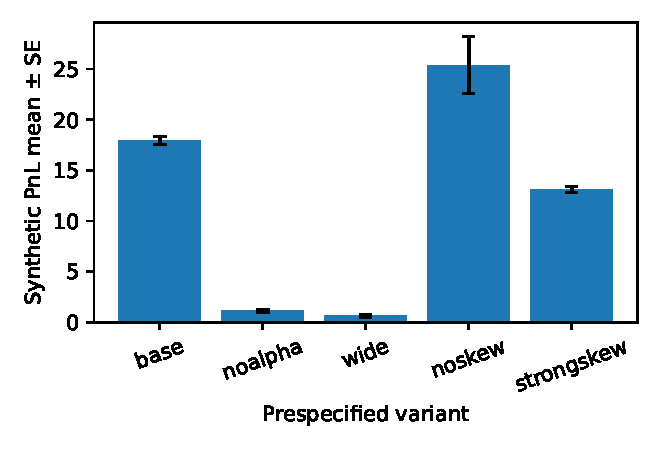
\includegraphics[width=\columnwidth]{figures/ablation.pdf}\caption{Primary synthetic ablation means and standard errors across 16 markets. Source: \texttt{primary.json}. Currency units over the simulated episode are not returns.}\end{figure}
Removing imbalance substantially reduces simulated PnL, consistent with the informed-flow design. Removing inventory skew trades increased position exposure for mean gains; the mean interval and sign test can disagree because of dispersion and sign balance. The held-out confirmation, regime results, fee outcomes and queue sweep are preserved in full rather than selecting only favorable cases. None establishes a profitable live strategy.

\begin{figure}[t]\centering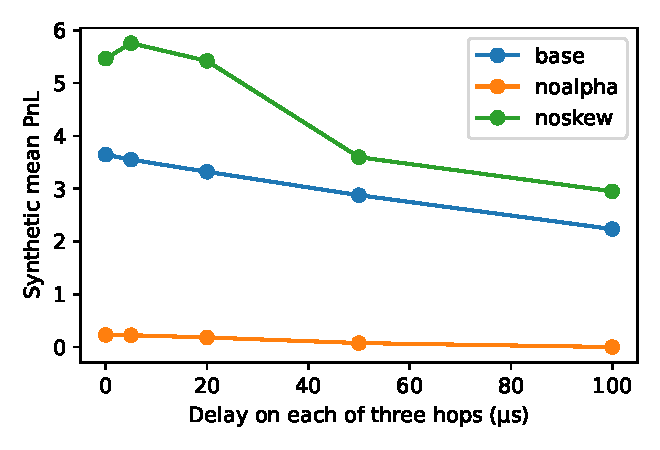
\includegraphics[width=\columnwidth]{figures/latency.pdf}\caption{Synthetic mean PnL versus delay applied to each of three hops. Source: \texttt{latency.json}. A generator response, not an empirical exchange threshold.}\end{figure}
The primary experiment's deterministic repeat exactly reproduces its JSON, including market digests. Histogram counts match their exported sample totals, and exported quantiles can be reconstructed within rounding. The reference benchmark requires identical final state digests. Full CTest, Python integration and fault-drill results are recorded separately in the artifact logs; skipped recorded-capture coverage is identified explicitly.

\section{Limitations and Reviewer Assessment}
Low in-memory latency does not establish low end-to-end exchange latency. Tails on a shared VM reflect scheduling, cache and calibration effects. Five repeated sessions and one host do not establish universal latency or hardware portability. Histogram binning loses individual sample order; no formal worst-case bound follows. The map/list reference is intentionally simple and excludes a tuned external engine.

Synthetic fills, same-generator holdouts, fee sensitivity and multiple regimes remain simulation evidence. Real exchange response formats, order rejection behavior, market impact, licensed historical datasets and profitability are outside this study. Statistical correction does not repair a misspecified generator. The prior claims of real LOBSTER/ITCH adapters, HJB optimality, formal invariants and historical mutation percentages are not carried forward without their required evidence.

The artifact is a useful systems contribution with modest algorithmic novelty. A credible submission needs a completed current literature comparison, stronger external baselines, independent artifact reproduction and a venue-specific contribution argument. An inspected copy of the original Avellaneda--Stoikov paper supports the theory attribution; direct access to scholarly indexes and current venue pages was blocked, so bibliography and current-call verification are incomplete. Author metadata is intentionally pending. The present recommendation is major revision before submission.

\section{Reproduction}
With CMake 3.31.10, Ninja 1.13.0, GCC 14, Python dependencies pinned in \texttt{research/requirements-lock.txt}, and TeX Live, run \texttt{bash research/reproduce.sh}. It builds, runs the required suites, executes the experiments, recomputes inference, generates figures and compiles this PDF. No exchange credentials or live orders are required. The branch remains local and no paper has been submitted.
\bibliographystyle{ieeetr}\bibliography{references}
\end{document}
